\documentclass[12pt, a4paper]{extarticle}
\usepackage{cmap}
\usepackage{amsfonts}
\usepackage[T2A]{fontenc}
\usepackage[utf8]{inputenc}
%\usepackage{mathtext}  
\usepackage{amsmath, amsfonts, amssymb}
\usepackage[russian]{babel}
\usepackage[body={17.5cm, 23.5cm},left=3cm, top=2cm, right=2cm]{geometry}
\usepackage{graphicx}
\usepackage{blindtext}
\usepackage{fancyhdr}
\usepackage{graphicx}
\usepackage{ragged2e}
\usepackage{epigraph}
\usepackage{misccorr}  
\usepackage{indentfirst} 
\usepackage{amsmath}
\usepackage{tabularx} 

\usepackage{fancyhdr} 
\usepackage{color}

\usepackage{makecell}
\usepackage{slashbox}

%\parindent{1.25cm} 
\graphicspath{images/}
\setcounter{tocdepth}{6}
\newcommand{\eps}{\varepsilon}
\newcommand{\re}{\operatorname{Re}}
\newcommand{\im}{\operatorname{Im}}

\newcommand{\lb}{\textquotedblleft}
\newcommand{\rb}{\textquotedblright}

\DeclareMathOperator{\sgn}{sgn}
\renewcommand{\labelitemi}{$-$}
\renewenvironment{itemize}[1][{---\hfil}]{\begin{list}{#1}{\topsep=0pt\parsep=0pt plus 1pt\itemsep=\parsep\leftmargin=0pt \itemindent=\parindent}\addtolength{\itemindent}{\labelwidth}}{\end{list}}

\numberwithin{equation}{section} 

\newtheorem{attachment}{\hspace{12cm}  Приложение}
\renewcommand{\theattachment}{\Alph{attachment}}
%\renewcommand{\newtheorem}{\Alph{attachment}}
%\newtheorem{Conjecture}{Conjecture}[section]

\usepackage{tocloft}
\renewcommand{\cftsecleader}{\cftdotfill{\cftdotsep}}

\begin{document}
\thispagestyle{empty} 
\medskip 

\begin{center} 
	\textbf{МИНОБРНАУКИ РОССИИ\\ 
		\vspace{0.5cm} 
		Федеральное государственное бюджетное образовательное\\ 
		учреждение высшего образования\\ 
		«Ярославский государственный университет им. П.Г. Демидова»}\\ 
	\vspace{0.5cm} 
	{Кафедра математического моделирования}\\ 
	\vspace{1.5cm} 
	
\end{center}
\begin{flushright} 
	Сдано на кафедру\\
	« 
	\underline{\phantom{aaa}} 
	» 
	\underline{\phantom{aaaaaaaaaaaaa}} 2019 г.\\ 
	Заведующий кафедрой\\
	\underline{\phantom{aaa}д. ф.-м. н., профессор\phantom{aaa}}\\ 
	\vspace{0.1cm} 
	\underline{\phantom{aaaaaaaaaaaaa}} С.А. Кащенко
\end{flushright}
\vspace{3cm} 
\begin{center} 
	Курсовая работа\\ 
	\vspace{0.5cm} 
	\textbf{Математическое моделирование движения транспортных потоков}\\ 
	\small{(Направление подготовки магистров 01.04.02 Прикладная математика и информатика)}
	\vspace{3cm} 
\end{center} 

\begin{flushright} 
	Научный руководитель\\ 
	\underline{\phantom{aaa}д. ф-м. н., доцент\phantom{aaa}}\\ 
	\vspace{0.1cm} 
	\underline{\phantom{aaaaaaaaaaaaa}} И.С. Кащенко\\ 
	« 
	\underline{\phantom{aaa}} 
	» 
	\underline{\phantom{aaaaaaaaaaaaa}} 2019 г.\\ 
	\vspace{0.5cm} 
	Студент группы \underline{\phantom{a}ПМИ-11МО\phantom{a}}\\ 
	\vspace{0.1cm} 
	\underline{\phantom{aaaaaaaaaaaaa}} М.А. Погребняк\\ 
	« 
	\underline{\phantom{aaa}} 
	» 
	\underline{\phantom{aaaaaaaaaaaaaa}}2019 г.\\ 
	\vspace{1cm} 
\end{flushright} 
\begin{center} 
	Ярославль 2019 г.
	\vspace{-1cm}  
\end{center} 


\justify 
\setlength{\parindent}{1.25cm} 
\newpage 
\thispagestyle{empty} 
\setcounter{page}{2} 
%\section*{Реферат}
%\vspace{\baselineskip}	

\newpage

\setcounter{page}{2}

%\thispagestyle{empty} 
\tableofcontents 
\newpage 

\section*{Введение}
\addcontentsline{toc}{section}{Введение}
\epigraph{\textit{Рано или поздно всякая правильная математическая идея находит применение в тои или ином деле.}}
{А. Н. Крылов}
В современном мире, где технологии и прогресс с огромной скоростью шагают вперёд, трудно представить, как человек смог бы обходится без мощного инструмента познания окружающей действительности под названием «математическое моделирование». С момента появления человека на земле математическое моделирование стало неотъемлемой частью его жизни. Необходимость в исследовании математических моделей прежде всего влияет на саму жизнь человека. Оно возникает, когда сами объекты или явления недоступны для изучения ввиду опасности, которую они представляют, удалены во времени и в пространстве или исследования связанны с большими материальными потерями и непредвиденными последствиями. Так или иначе математическое моделирование имеет огромную важность в жизни человека и никогда не потеряет свою актуальность.

В настоящее время, в связи с развитием компьютерной техники и постоянным совершенствованием программного обеспечения, математическое моделирование развивается быстрыми темпами. Возрастающие потребности в различных сферах общества, например, разработка и управление техническими устройствами, анализ экономических и социальных процессов, способствуют этому. Все естественные и общественные науки, использующие математический аппарат, по сути занимаются математическим моделированием: заменяют реальный объект его аналогом, отражающим в математической форме важнейшие его свойства, а затем изучают его.  Результаты таких исследований очень содержательны и применимы в повседневной жизни. Математическая модель выражает существенные черты объекта или процесса языком уравнений и других математических средств. 

Метод математического моделирования занимает одно из ведущих мест в исследованиях сложных явлений и процессов, так как позволяет количественно и качественно описать наиболее существенные связи между переменными в системе и применить достаточно развитый математический аппарат и программные средства для анализа явлений, а также для их прогнозирования и управления этими процессами. 

Математическое моделирование очень часто встречается в физике, ведь не зря математику называют языком физики. Эти науки всегда тесно связаны и взаимно обогащают друг друга идеями и методами. Хотя физика и считается наукой о природе, изучающая простейшие и вместе с тем наиболее общие свойства материального мира, но она базируется на моделях объектов материального мира. Поэтому метод математического моделирования изначально зародился в физике, точнее, в математической физике, а затем постепенно начал проникать и в другие науки, где со временем стал очень востребован. Раньше из обширного математического аппарата физики применяли в основном аналитические и полуаналитические методы и приёмы Сейчас все чаще обращаются к математическому моделированию, когда исследуемый физический процесс описывается некоторой математической моделью, представляющей собой систему дифференциальных или интегро-дифференциальных уравнений математической физики. Изучая какие-либо физические явления, исследователь прежде всего создаёт его математическую идеализацию или, другими словами, математическую модель, то есть, пренебрегая второстепенными характеристиками явления, он записывает основные законы, управляющие этим явлением, в математической форме и очень часто эти законы выражаются в виде дифференциальных уравнений. Для составления математической модели в виде дифференциальных уравнений нужно, как правило, знать только локальные связи и не нужна информация обо всем физическом явлении в целом.

Современные компьютерные технологии позволили подойти к решению проблемы математического моделирования транспортных потоков. Основы математического моделирования, закономерностей дорожного движения были заложены в 1912 году русским учёным, профессором Г.Д. Дубелиром. В своей книге «Городские улицы и мостовые» \cite{Street} он положил начало развитию такой отрасли как моделирование транспортных потоков. За прошедший век непрерывных исследований выработалось много хороших моделей, которые помогают сегодня строить качественные и быстрые дороги и регулировать транспортные потоки. Но проблема транспортных потоков никуда не уходит, а на оборот только возрастает в связи с увеличением численности людей на земле, строительством и расширением городов и сообщений между ними и как следствие развитием и модернизацией транспорта.  Транспорт— одна из ключевых систем городского организма, которую по важности уместно сравнить с кровоснабжением. Именно транспорт позволяет городу в полной мере выполнять связующую, коммуникационную и обеспечивающую функции. Тема транспорта касается практически каждого городского жителя, и тем важнее становятся усилия по систематизации управления дорожным движением на транспортной сети городов, ведь без грамотно проработанной транспортной модели, управлять городскими потоками практически, невозможно. Например, в определённом месте городской магистрали систематически возникают автомобильные пробки. Если модель транспортной системы отсутствует, высока вероятность принятия ошибочного решения, результатом которого станет перенос пробки на новое место или создание новых автомобильных пробок. Создавая подобные модели, можно планировать транспортные системы современных городов. Изменения в одной части такой системы приводят к появлению изменений в других ее частях. Насколько увеличится автомобильный поток, если сделать дорогу более широкой? Почему автомобильная пробка регулярно образуется на конкретном перекрёстке? Какой потенциал создаст развитие системы городского общественного транспорта для изменения застройки в черте города? Что случится, если внести изменения в режим работы определённого светофора? Ответить на все эти, а также многие другие вопросы позволяет моделирование транспортной системы. Одна из наиболее трудных проблем, стоящих перед исследователем
организации движения — это превращение реальной дорожно-транспортной обстановки, включающей водителей, автомобили, устройства регулирования движения и дорогу, в набор математических символов и зависимостей, воспроизводящих их поведение. Именно тут математическое моделирование является основой, которая позволяет рассматривать подобные взаимодействия в целом. Решение задач моделирования транспортных потоков и внедрение этих технологий позволяет значительно улучшить ситуацию на проезжей части дороги, снизить тенденцию к образованию транспортных пробок, перегрузке или недогрузке отдельных линий и узлов транспортной сети, снижению уровня аварийности, а также помогает решать и экологические проблемы.

\newpage
\section{Постановка задачи} 
Используя теоретические подходы исследования движения транспортных потоков, составить математическую модель для описания движения транспортных потоков. Данная модель должна представлять из себя набор дифференциальных уравнений и иметь практическую значимость. Полученную модель необходимо исследовать, используя компьютерные технологии.   

\newpage
\section{Общие положения моделирования движения транспортных потоков}
Научное исследование транспортных потоков началось в 1910-х годах прошлого века и продолжает развиваться в наши дни. В условиях стремительного расширения городов и развития их инфраструктуры становится всё более актуальным моделирование потоков автомобильного транспорта. За более чем вековую историю исследований было создано и применено множество различных теорий и методов, а так же было создано множество различных моделей. Всё множество таких моделей можно разделить на три группы, в зависимости от основного подхода, используемого при моделировании.

Первая группа - это \textbf{вероятностные} модели. В этих моделях транспортный поток рассматривается как результат взаимодействия транспортных средств на элементах транспортной сети.
Такой подход используют стохастические модели.

Вторая группа - это \textbf{макроскопические} модели. В таких моделях автомобильная среда рассматривается на трассе как нечто цельное. Обычно её уподобляется какому-либо физическому потоку. Существует целый ряд газокинетических, гидродинамических моделей, использующих такой подход.

Третья группа - это \textbf{микроскопические} модели. В этих моделях каждый автомобиль рассматривается как отдельная частица со своей скоростью и конечной целью. К таким моделям можно отнести модели, основанные на теории клеточных автоматов и модели, основанные на принципе следования за лидером.

В данной работе рассматриваются различные модели, построенные с использованием микроскопических методов, а именно подход, основанный на движении транспортных средств друг за другом {\it(follow the leader)}.

Под \textbf{транспортным средством} будем понимать {\it техническое устройство для перевозки людей и/или грузов} \cite{TrafficFlow}.

Под \textbf{транспортным потоком} будем понимать {\it количество единиц транспортных средств одного вида транспорта, проследовавших определённый участок пути в течение установленного промежутка времени} \cite{TrafficFlow}.

В качестве транспортного средства рассмотрим автомобиль и будем называть его \textbf{лидером}, если за ним есть другой автомобиль, или \textbf{преследователем}, если перед ним есть другой автомобиль. Причём, один и тот же автомобиль может являться одновременно и преследователем для впереди идущего, и лидером для позади идущего (рис. \ref{car_following}). 

\begin{figure}[h!]  
	\begin{center}
		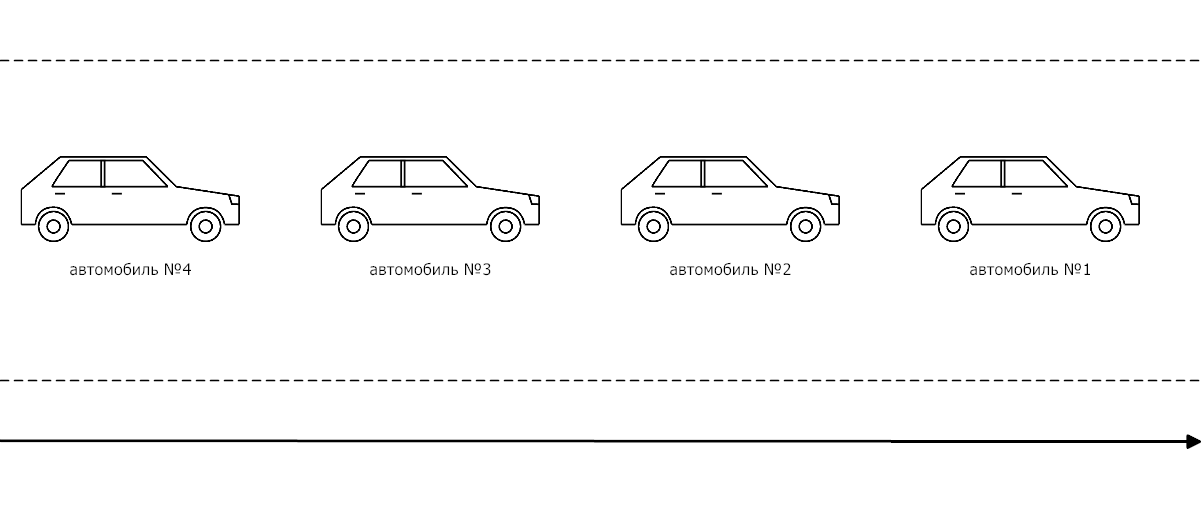
\includegraphics[keepaspectratio,width=160mm,height=70mm]{Images/car_following.png}
	\end{center}
	\caption{Автомобили, следующие друг за другом.}
	\label{car_following}
\end{figure}

Рассмотрим парадигму автомобиля, которая основана на очень простом правиле и уже довольно давно известна в литературе. Так как автомобили следуют друг за другом, преследователь всегда пытается максимизировать свою скорость с двумя ограничениями: ограничением ускорения и ограничением безопасности. Впервые данная парадигма была высказана ещё в 1975 \cite{GippsModel} и математически выглядит следующим образом:

\begin{equation} \label{following_paradigm}
v_f(t) = \min(v_f^d(t), v_f^s(t)),
\end{equation}
где $v_f(t)$ - скорость преследователя в момент времени $t$, $v_f^d(t)$ - максимальная возможная скорость с \textbf{ограничением ускорения} (demand speed), $v_f^s(t)$ - максимальная возможная скорость с \textbf{ограничением безопасности} (supply speed).

Под ограничение ускорения стоит понимать физические ограничения скорости и ускорения транспортного средства, а также условия комфорта, необходимые водителю. Оно описывает траекторию транспортного средства, которое свободно разгоняется до максимальной желаемой скорости при отсутствии впереди идущих транспортных средств. Это не всегда постоянное значение: например, оно может зависеть от скорости автомобиля. Ограничение безопасности - это то, как траектория транспортного средства зависит от впереди идущего транспортного средства (лидера).

\section{Модель свободного движения}

Для начала рассмотрим простую ситуацию, когда на дороге есть всего один автомобиль, для которого нет никаких ограничений, за исключением технических характеристик транспортного средства. В такой ситуации парадигму автомобиля \eqref{following_paradigm} можно записать следующим образом:

\begin{equation} \label{following_paradigm_alone}
v_f(t) = v_f^d(t),
\end{equation}
то есть автомобиль свободно разгонится до максимально желаемой скорости и будет продолжать с ней движение. Такое поведение будем называть свободным движением. 

Для описания свободного движения можно использовать обыкновенное дифференциальное уравнение вида: 
\begin{equation} \label{free_drive_with_initial_conditions}
\begin{cases}
\begin{split}
\ddot{x}&(t) = a\left( 1-\left( \dfrac{\dot{x}(t)}{v_{max}}\right)^\delta \right) \\
&x(0)=x_0, \quad \dot{x}(0)=v_{0}
\end{split}
\end{cases}.
\end{equation}
Из уравнения \eqref{free_drive_with_initial_conditions} видно, что свободное движение характеризуется максимально допустимой (желаемой) скоростью $v_{max}$, начальной скоростью $v_{0}$, начальным положением транспортного средства $x_0$, максимальным ускорением $a$ и показателем степени $\delta$, определяющим, как ускорение уменьшается с ростом скорости.

Без потери общности можно рассматривать модель \eqref{free_drive_with_initial_conditions} при линейном уменьшении ускорения с ростом скорости, что соответствует $\delta=1$.

У системы \eqref{free_drive_with_initial_conditions} существует решение в явном виде:
\begin{equation*}
x(t) = \dfrac{1}{a}\left(av_{max}t+v_{max}^2e^{-\frac{at}{v_{max}}}-v_{max}^2-v_{max}v_0e^{-\frac{at}{v_{max}}}+v_{max}v_0+ax_0\right). 
\end{equation*}
Из точного решения хорошо видна динамика автомобиля в нулевой момент времени $t=0$ в случаях, когда $v_0=v_{max}$ и $v_0=0$. Ускорение в начальный момент времени описывает равенство $x''(0)=a-\dfrac{av_0}{v_{max}}$, из которого видно, что при $v_0=v_{max}$ ускорения нет, а при $v_0=0$ автомобиль начинает движение с максимальным ускорением. Такое поведение полностью согласуется с динамикой реального транспортного средства.

На рисунке \eqref{free_drive_without_stop} изображены графики скорости и расстояния для свободно двигающегося автомобиля.
\begin{figure}[h!]
	\begin{center}
		\begin{minipage}[h!]{0.48\linewidth}
			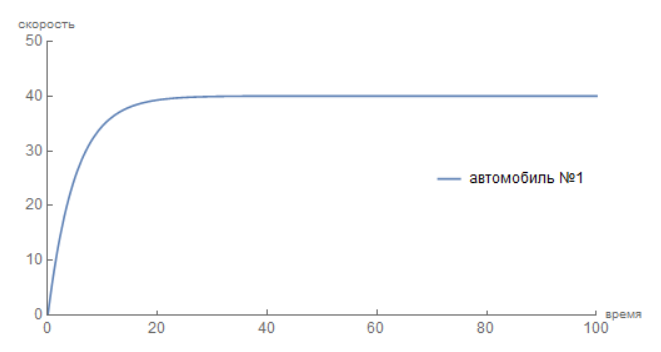
\includegraphics[width=1\linewidth,height=0.2\textheight]
			{Images/free_drive_speed.png}
		\end{minipage}
		\hfill 
		\begin{minipage}[h!]{0.48\linewidth}
			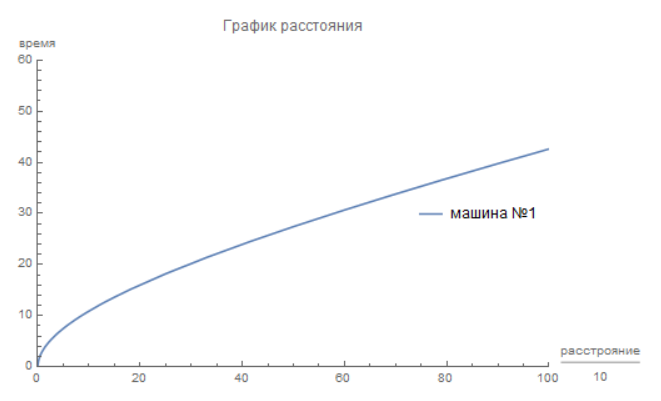
\includegraphics[width=1\linewidth,height=0.2\textheight]
			{Images/free_drive_distance.png}
		\end{minipage}
		\caption{Графики изменения скорости (слева) и расстояния (справа) для автомобиля при свободном движении без остановки с параметрами: $a=8$, $v_{max}=40$, $x_0=0$, $v_0=0$.}
		\label{free_drive_without_stop}
	\end{center}
\end{figure}

Как видно из графиков, автомобиль, разогнавшись до максимальной допустимой (желаемой) скорости, бесконечно двигается вперёд. Данная модель отлично описывает момент старта автомобиля, его разгон и движение с постоянной скоростью. Под стартом автомобиля будем понимать момент начала разгона. В более жизненных ситуациях присутствуют процессы обратные разгону и старту - торможение и остановка.

Для описания остановки автомобиля рассмотрим следующее дифференциальное уравнение: 
\begin{equation} \label{stop_drive_with_initial_conditions}
\begin{cases}
\begin{split}
\ddot{x}&(t) = q\left( v_{min} - \dot{x}(t)\right) \\
&x(0)=x_0, \quad \dot{x}(0)=v_0
\end{split}
\end{cases}.
\end{equation}
Из уравнения \eqref{stop_drive_with_initial_conditions} видно, что остановка характеризуется минимальной (желаемой) скоростью $v_{min}$, начальной скоростью $v_{0}$, начальным положением транспортного средства $x_0$, коэффициентом торможения $q$. Под минимальной скоростью будем понимать такую скорость до которой водитель транспортного средства хочет снизить свою текущую скорость. Это не обязательно нулевая величина, в некоторых случаях водитель не хочет останавливаться полностью, а хочет лишь снизить скорость.

Аналогично системе, описывающей ускорение, система \eqref{stop_drive_with_initial_conditions} также имеет решение в явном виде:
\begin{equation*}
x(t) = \dfrac{1}{q}\left(av_{min}t+v_{min}e^{-qt}-v_{min}-v_0e^{-qt}+v_0+qx_0\right) 
\end{equation*}
Ускорение в начальный момент времени описывает равенство $x''(0)=q(v_{min}-v_0)$, из которого видно, что при $v_0=v_{min}$ торможения нет, а при $v_0=0$ автомобиль начинает тормозить с к коэффициентом $-qv_0$. Данное поведение также согласуется с динамикой реального транспортного средства.

Уравнения \eqref{free_drive_with_initial_conditions} и  \eqref{stop_drive_with_initial_conditions} описывают два разных вида движения. Для получения общей модели, описывающей оба этих вида движения, необходимо объединить их в одну. Предположим, что в нулевой момент времени происходит первая фаза движения - старт автомобиля и его разгон. Затем с некоторого момента времени $t_s$ (stop time) происходит вторая фаза движения - автомобиль начинает тормозить. Введём две релейные функции $R_{a}(t)$ и $R_{b}(t)$, вида:  

\begin{equation*} 
R_{a}(t)=
\begin{cases}
\begin{split}
&1, \quad t<t_{s} \\
&0, \quad t\geq t_{s}
\end{split}
\end{cases},
\qquad
R_{b}(t)=
\begin{cases}
\begin{split}
&0, \quad t<t_{s} \\
&1, \quad t\geq t_{s}
\end{split}
\end{cases},
\end{equation*}
Релейная функция $R_{a}(t)$ "включается"{}, когда автомобиль находится в фазе разгона (acceleration phase) и "выключается"{}, когда автомобиль переходит в фазу торможения (braking phase). Функция $R_{b}(t)$ наоборот - "выключается"\ в фазе разгона и "включается"\ в фазе торможения. Функцию $R_{a}(t)$ можно выразить через $R_{b}(t)$ следующим образом $R_{a}(t) = (1-R_{b}(t))$. Обозначим $R_{a}(t)$ как $R(t)$ и получим релейную функцию, которая объединяет два вида движения.

\begin{equation} \label{relay_function}
R(t)=
\begin{cases}
\begin{split}
&1, \quad t<t_{s} \\
&0, \quad t\geq t_{s}
\end{split}
\end{cases}.
\end{equation}

С помощью полученной релейной функции \eqref{relay_function} объединим модели \eqref{free_drive_with_initial_conditions} и  \eqref{stop_drive_with_initial_conditions} и получим полную модель свободного движения:
\begin{equation} \label{free_drive_model}
\begin{cases}
\begin{split}
\ddot{x}(t) = &R(t) \left[ a\left(\dfrac{v_{max}-\dot{x}(t)}{v_{max}} \right)\right] + (1-R(t)) \bigg[ q\left( v_{min} - \dot{x}(t)\right) \bigg]  \\
&x(0)=x_0, \quad \dot{x}(0)=v_{0}
\end{split}
\end{cases}.
\end{equation}
Обозначения, используемые в модели \eqref{free_drive_model}, приведены в таблице \ref{free_drive_parameters}.
\begin{table}[h!]
	\caption{Физическое значение параметров модели \eqref{free_drive_model}}
	\label{free_drive_parameters}
	\begin{center}
		\begin{tabularx}{\textwidth}{p{0.15\linewidth}p{0.85\linewidth}}			
			\hline
			\rule{0cm}{0,5cm}
			Параметр &  Физическое значение \\ 
			[3pt]\hline
			$a$ & коэффициент максимального ускорения\\
			$q$ & коэффициент торможения\\ 
			$v_{max}$ & максимальная скорость\\
			$v_{min}$ & минимальная скорость\\ 
			$x_0$ & начальное положение\\
			$v_0$ & начальная скорость\\ 
			$R(t)$ & релейная функция, переключающая фазы движения  \\ 
			\hline
		\end{tabularx}
	\end{center}
\end{table}

На рисунке \eqref{free_drive_with_stop} изображены графики скорости и расстояния для свободно двигающегося автомобиля с остановкой.

\begin{figure}[h!]
	\begin{center}
		\begin{minipage}[h!]{0.48\linewidth}
			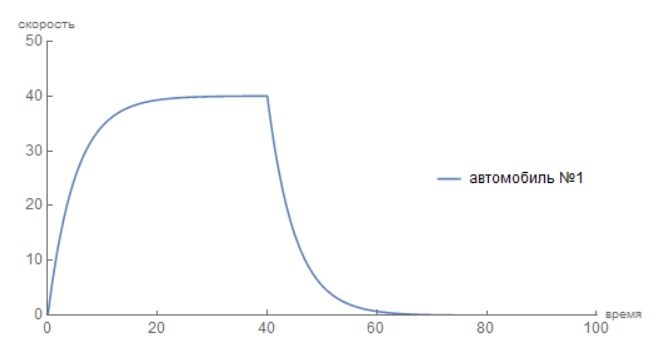
\includegraphics[width=1\linewidth,height=0.2\textheight]
			{Images/free_drive_speed_with_stop.png}
		\end{minipage}
		\hfill 
		\begin{minipage}[h!]{0.48\linewidth}
			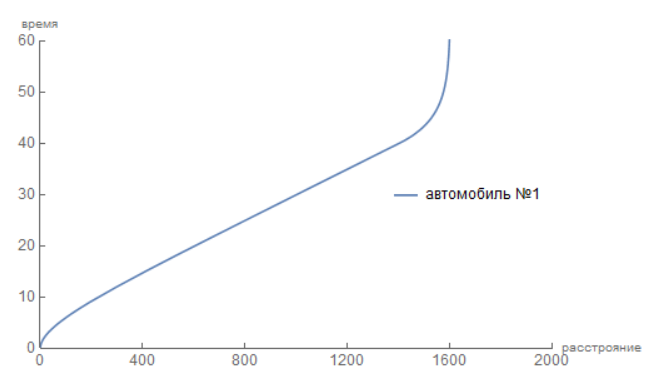
\includegraphics[width=1\linewidth,height=0.2\textheight]
			{Images/free_drive_distance_with_stop.png}
		\end{minipage}
		\caption{Графики изменения скорости (слева) и расстояния (справа) для автомобиля при свободном движении без остановки с параметрами: $a=8$, $q=0.2$, $v_{max}=40$, $v_{min}=0$, $t_s=40$, $x_0=0$, $v_0=0$.}
		\label{free_drive_with_stop}
	\end{center}
\end{figure}

Из графиков видно, что автомобиль, разогнавшись до максимальной допустимой (желаемой) скорости, двигается с ней до наступления времени торможения. Затем автомобиль начинает тормозить до минимальной желаемой скорости и продолжает с ней движение или же, если минимальная скорость равна нулю ($v_{min}=0$), как на графиках \eqref{free_drive_with_stop}, останавливается.
 
Таким образом была получена модель \eqref{free_drive_model}, которая описывает все значимые фазы движения одного автомобиля, а именно разгон, само движение и торможение. Даная модель не учитывает внешних факторов, которые оказывают влияние на движение автомобиля, она зависит лишь от технических характеристик транспортного средства и от самого водителя. Эта модель подходит для описания динамики первого автомобиля в потоке. На остальные автомобили большое влияние оказывают впереди идущие транспортные средства, поэтому они вынуждены двигаться учитывая движение лидера.

\section{Модель следования за лидером}

Рассмотрим несколько автомобилей и занумеруем их индексом $n$ в соответствии с их порядковым номером на дороге. Предполагается, что ускорение $n$-ого автомобиля определяется состоянием соседних автомобилей, а именно наибольшее влияние оказывает непосредственно впереди идущий автомобиль (лидер).

Первая модель, основанная на принципе следования за лидером была разработана в 50-х годах прошлого века и предполагала, что каждый водитель адаптирует свою скорость к скорости лидирующего автомобиля:

\begin{equation} \label{follow_the_leader_first_model}
\ddot{x}_n(t) = \dfrac{1}{\gamma} (\dot{x}_{n-1}(t) - \dot{x}_{n}(t)), 
\end{equation}
где $\gamma$ - время адаптации водителя.

Данное уравнение было получено в работе Пайпса (Pipes) \cite{FirstFollowTheLeaderModel}. Модель, построенная на основе данного уравнения, является простой и плохо описывает свойства реального транспортного потока.

В работе \cite{RefineFirstFollowTheLeaderModel} была предложена модификация уравнения \eqref{follow_the_leader_first_model}. В левую часть уравнения была введена задержка аргумента по времени $\tau$, которая отражает время реакции водителей на изменение скорости лидирующего автомобиля. 

\begin{equation*}
\ddot{x}_n(t+\tau) = \dfrac{1}{\gamma} (\dot{x}_{n-1}(t) - \dot{x}_{n}(t)).
\end{equation*}
Произведя замену времени получим следующие уравнение:
\begin{equation} \label{follow_the_leader_with_two_delay}
\ddot{x}_n(t) = \dfrac{1}{\gamma} (\dot{x}_{n-1}(t-\tau) - \dot{x}_{n}(t-\tau)).
\end{equation}

Уравнение \eqref{follow_the_leader_with_two_delay} содержит два запаздывания в правой части, то есть ускорение автомобиля зависит от разности скоростей, которые были у текущего и впереди идущего автомобилей $\tau$ времени назад.

Упростим уравнение \eqref{follow_the_leader_with_two_delay}, оставив в правой части только одно запаздывание у уменьшаемого, таким образом ускорение автомобиля будет зависеть от его текущей скорости и скорости впереди идущего автомобиля $\tau$ времени назад. Множитель $\dfrac{1}{\gamma}$ будем интерпретировать как коэффициент мощности $d$, характеризующий мощность двигателя автомобиля. С учётом проведённых модификаций уравнение примет вид:

\begin{equation} \label{follow_the_leader_with_delay}
\ddot{x}_n(t) = d_{n} (\dot{x}_{n-1}(t-\tau) - \dot{x}_{n}(t)).
\end{equation}

Без потери общности будем считать, что все автомобили имеют одинаковые технические характеристики $d_n = d$, а все водители одинаково оценивают дорожную ситуацию и реагируют на её изменения с одинаковой скоростью $\tau = const$.

Уравнение \eqref{follow_the_leader_with_delay} можно проинтегрировать и рассматривать модель, которая описывает скорость и зависит от положения самого автомобиля и положения лидера. Данный подход подробно описан в \cite{Course}, в данной работе будем рассматривать уравнение в исходном виде. 

Запишем общую модель движения транспортного потока. Движение первого автомобиля будет описывать ранее выведенное уравнение \eqref{free_drive_model}, остальные автомобили будет двигаться согласно разностному уравнению \eqref{follow_the_leader_with_delay}.

\begin{equation} \label{follow_the_leader_full_model}
\begin{cases}
\begin{split}
\ddot{x}_1(t) = &R(t) \left[ a\left(\dfrac{v_{max}-\dot{x}_1(t)}{v_{max}} \right)\right] + (1-R(t)) \bigg[ q\left( v_{min} - \dot{x}_1(t)\right) \bigg]  \\
&x_{1}(0)=x_0, \quad \dot{x}_{1}(0)=v_{0}\\
\ddot{x}_{n}(t) = &d(\dot{x}_{n-1}(t-\tau)-\dot{x}_{n}(t)) \\
&x_n(0)=x_0-(n-1)\lambda, \quad \dot{x}_n(0)=v_{n}, \quad t \in [-(n-1)\tau,0]
\end{split}
\end{cases}.
\end{equation}
Обозначения, использующиеся в системе \eqref{follow_the_leader_full_model}, приведены в таблице \ref{follow_the_leader_full_model_parameters}.
\begin{table}[h!]
	\caption{Физическое значение параметров уравнения \eqref{follow_the_leader_full_model}}
	\label{follow_the_leader_full_model_parameters}
	\begin{center}
		\begin{tabularx}{\textwidth}{p{0.15\linewidth}p{0.85\linewidth}}			
			\hline
			\rule{0cm}{0,5cm}
			Параметр &  Физическое значение \\ 
			[3pt]\hline
			$a$ & коэффициент максимального ускорения\\
			$q$ & коэффициент торможения\\ 
			$v_{max}$ & максимальная скорость\\
			$v_{min}$ & минимальная скорость\\ 
			$x_0$ & начальное положение\\
			$v_0$ & начальная скорость\\ 
			\hline
		\end{tabularx}
	\end{center}
\end{table}


На рисунке \eqref{follow_the_leader} изображены графики скорости и расстояния для нескольких автомобилей, движущихся друг за другом.

\begin{figure}[h!]
	\begin{center}
		\begin{minipage}[h!]{0.48\linewidth}
			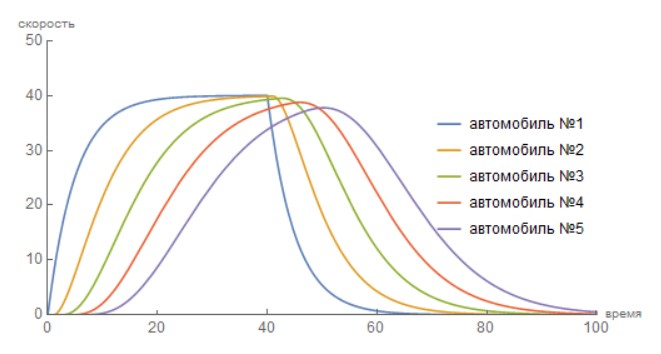
\includegraphics[width=1\linewidth,height=0.2\textheight]
			{Images/simple_model_speed.png}
		\end{minipage}
		\hfill 
		\begin{minipage}[h!]{0.48\linewidth}
			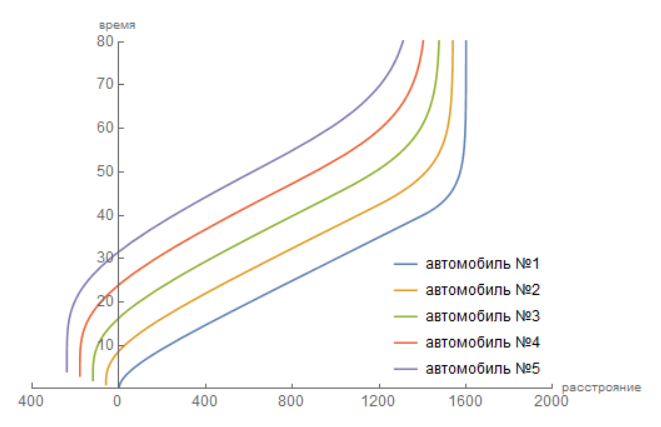
\includegraphics[width=1\linewidth,height=0.2\textheight]
			{Images/simple_model_distance.png}
		\end{minipage}
		\caption{Графики изменения скорости (слева) и расстояния (справа) для транспортного потока с остановкой с параметрами: $\tau=1$, $a=8$, $q=0.2$, $v_{max}=40$, $v_{min}=0$, $\lambda=40$, $d=0.2$, $t_s=40$, $x_0=0$, $v_0=0$.}
		\label{follow_the_leader}
	\end{center}
\end{figure}

Из графиков видно, что автомобили, разгоняются до максимальной желаемой скорости и двигаются до момента времени $t_s$, начиная с которого, первый автомобиль тормозит и останавливается. Остальные автомобили, повторяя динамику первого автомобиля, так же останавливаются. Все движение происходит с сохранением безопасной дистанции между автомобилями, что соответствует реальному транспортному потоку, так как сокращение безопасного расстояния подразумевает появление аварийной ситуации.

Результаты исследования модели \eqref{follow_the_leader_full_model} совпадают с  результатами исследований моделей \eqref{follow_the_leader_with_two_delay} и проинтегрированной \eqref{follow_the_leader_full_model} из работ \cite{RefineFirstFollowTheLeaderModel} и \cite{Course} соответственно. С помощью регулировки коэффициентов в моделях можно добиться полной идентичности решений. Из этого можно сделать вывод, что все три модели одинаково описывают динамику движения транспортных средств и могут быть в равной мере использованы для моделирования движения транспортных потоков.

\section{Модель Газиса}

Группа инженеров из компании «Дженерал моторс» (General Motors) в своей работе \cite{GazisModel} предложила дополнительную модификацию для уравнения  \eqref{follow_the_leader_with_two_delay}. Основной этой модификации является идея рассмотреть вместо постоянного коэффициента $\dfrac{1}{\gamma}$ динамическую величину $S(t)$, которую можно интерпретировать как коэффициент чувствительности. 

Коэффициент чувствительности $S(t)$ характеризует скорость реакции водителя к изменению скорости лидера и зависит от скорости и текущей дистанции до лидера. Чувствительность возрастает при уменьшении дистанции до лидера, таким образом коэффициент $S(t)$ можно представить в виде:

\begin{equation*}
S(t) = \dfrac{\eta_{l,m}\dot{x}_n^{m_1}(t)}{(x_{n-1}(t-\tau)-x_n(t-\tau))^{m_2}},
\end{equation*}
где $\eta$ - константа, характеризующая движение, а $m_1$ и $m_2$ - эмпирически подбираемые константы, характеризующие движение. Данный коэффициент был получен в работе Газиса \cite{GazisModel}, в честь которого и была названа модель, полученная с учётом сделанных преобразований:   
\begin{equation} \label{gazis_model}
\ddot{x}_n(t) = \dfrac{\eta_{l,m}\dot{x}_n^{m_1}(t)}{(x_{n-1}(t-\tau)-x_n(t-\tau))^{m_2}} (\dot{x}_{n-1}(t-\tau) - \dot{x}_{n}(t-\tau)).
\end{equation}

Изучение модели, полученной Газисом, в исходном виде описано в работах \cite{StudyingGazisModel_1},  \cite{StudyingGazisModel_2} и  \cite{StudyingGazisModel_3}. При значениях параметров $m_1 \approx 0.8$, $m_2 \approx 2.8$ \cite{StudyingGazisModel_1} или $m_1 = 0.953$, $m_2 = 3.05$ \cite{StudyingGazisModel_2}, \cite{StudyingGazisModel_3} получаются результаты наиболее схожие с реальными данными.

Дополним уравнение Газиса \eqref{gazis_model} уравнением первого автомобиля \eqref{free_drive_model} и рассмотрим полученную модель движения транспортного потока:

\begin{equation} \label{full_gazis_model}
\begin{cases}
\begin{split}
\ddot{x}_1(t) = &R(t) \left[ a\left(\dfrac{v_{max}-\dot{x}_1(t)}{v_{max}} \right)\right] + (1-R(t)) \bigg[ q\left( v_{min} - \dot{x}_1(t)\right) \bigg]  \\
&x_{1}(0)=x_0, \quad \dot{x}_{1}(0)=v_{0}\\
\ddot{x}_n(t) = & \dfrac{\eta_{l,m}\dot{x}_n^{m_1}(t)}{(x_{n-1}(t-\tau)-x_n(t-\tau))^{m_2}} (\dot{x}_{n-1}(t-\tau) - \dot{x}_{n}(t-\tau)) \\
&x_n(0)=x_0-(n-1)\lambda, \quad \dot{x}_n(0)=v_{n}, \quad t \in [-(n-1)\tau,0]
\end{split}
\end{cases}.
\end{equation}

Полученные модели \eqref{gazis_model} и \eqref{full_gazis_model} очень сильно зависят от эмпирически подбираемых констант $m_1$ и $m_2$. При неудачном выборе данных констант решения не согласуются с реальными данными. На рисунках \ref{gazis_model_good} и \ref{gazis_model_bad} изображены графики решений для "удачного" и "неудачного" выбора параметров. 
\begin{figure}[h!]
	\begin{center}
		\begin{minipage}[h!]{0.48\linewidth}
			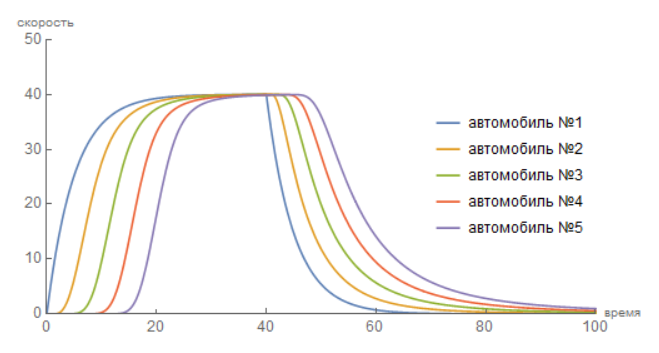
\includegraphics[width=1\linewidth,height=0.2\textheight]
			{Images/gazis_model_good_speed.png}
		\end{minipage}
		\hfill 
		\begin{minipage}[h!]{0.48\linewidth}
			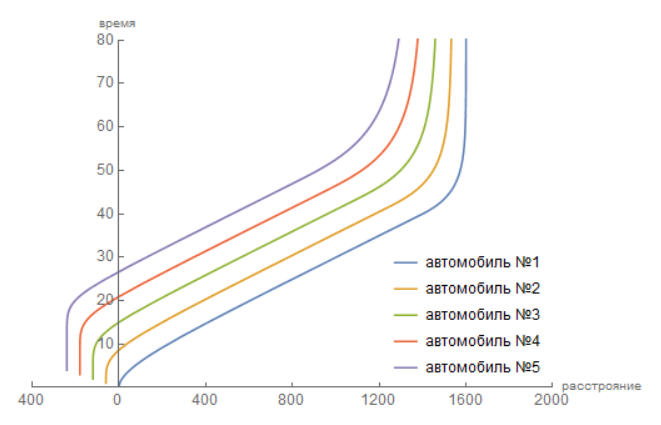
\includegraphics[width=1\linewidth,height=0.2\textheight]
			{Images/gazis_model_good_distance.png}
		\end{minipage}
		\caption{Графики изменения скорости (слева) и расстояния (справа) для модели Газиса с "удачным" выбором параметров: $\tau=1$, $a=8$, $q=0.2$, $v_{max}=40$, $v_{min}=0$, $\lambda=40$, $t_s=40$, $x_0=0$, $v_0=0$, $\eta=0.4$, $\boldsymbol{m_1=0.4}$, $\boldsymbol{m_2=0.3}$}
		\label{gazis_model_good}
	\end{center}
\end{figure}

\begin{figure}[h!]
	\begin{center}
		\begin{minipage}[h!]{0.48\linewidth}
			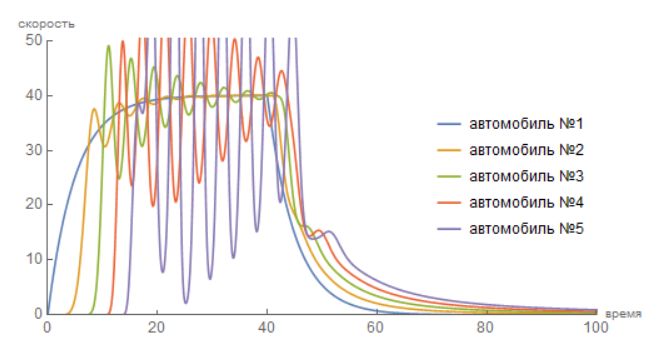
\includegraphics[width=1\linewidth,height=0.2\textheight]
			{Images/gazis_model_bad_speed.png}
		\end{minipage}
		\hfill 
		\begin{minipage}[h!]{0.48\linewidth}
			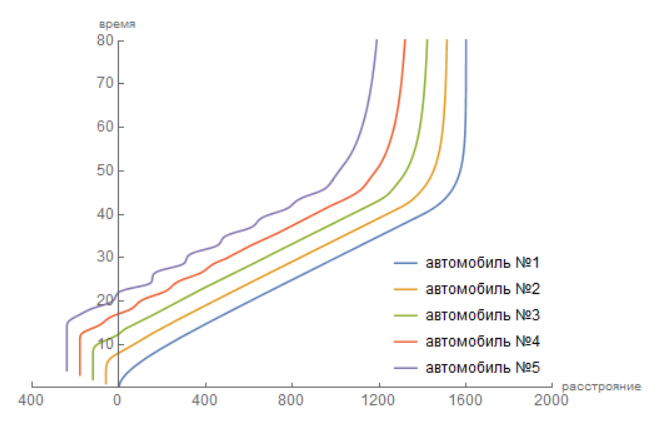
\includegraphics[width=1\linewidth,height=0.2\textheight]
			{Images/gazis_model_bad_distance.png}
		\end{minipage}
		\caption{Графики изменения скорости (слева) и расстояния (справа) для модели Газиса с "неудачным" выбором параметров: $\tau=1$, $a=8$, $q=0.2$, $v_{max}=40$, $v_{min}=0$, $\lambda=40$, $t_s=40$, $x_0=0$, $v_0=0$, $\eta=0.4$, $\boldsymbol{m_1=0.7}$, $\boldsymbol{m_2=0.3}$}
		\label{gazis_model_bad}
	\end{center}
\end{figure}

Графики на рисунке \ref{gazis_model_good} демонстрируют хорошую ситуацию, когда решения согласуются с реальным поведением транспортных средств на дороге. Графики на рисунке \ref{gazis_model_bad} показывают плохую ситуацию. Скорость некоторых автомобилей с некоторого момента времени начинает сильно колебаться с большой амплитудой и не только превышает допустимую скорость, но и в некоторых случаях падает почти до нуля. Такое поведение невозможно в реальной жизни.

Из результатов исследования можно сделать вывод, что ни "частая" модель Трайбера \eqref{gazis_model} ни модель Трайбера, дополненная уравнением движения первого автомобиля \eqref{full_gazis_model}, не подходят для моделирования движения автомобилей. Большая зависимость от правильного выбора параметров $m_1$ и $m_2$ и несвязанность этих параметров с каким-то физическими величинами очень усложняет моделирование и не гарантирует получение правильной динамики движения транспортных потоков. 

\section{Модель Трайбера}

\subsection{Классическая модель Трайбера}
\begin{equation*}
\begin{cases}
\begin{split}
&\dot{x}_n(t) = v_n(t), \\
&\dot{v}_n(t)=f(t, v_n,v_{n-1},x_{n-1}-x_n)
\end{split}
\end{cases}.
\end{equation*}

\begin{equation*}
\begin{cases}
\begin{split}
&\dot{x}_n(t) = v_n(t), \\
&\dot{v}_n(t)=\left[ a\left( 1-\left( \dfrac{v_n(t)}{v_{max}}\right) \right)\right] - a\left( \dfrac{s^*(v_n,\Delta v_n)}{s_n}\right)^2
\end{split}
\end{cases}.
\end{equation*}


\begin{equation*}
\begin{cases}
\begin{split}
&\dot{x}_n(t) = v_n(t), \\
&\dot{v}_n(t)=\left[ a\left( 1-\left( \dfrac{v_n(t)}{v_{max}}\right) \right)\right]-a\left( \dfrac{\sigma_0+\sigma_1\sqrt{\frac{v_n}{v_{max}}}+Tv_n+\frac{v_n(v_n-v_{n-1})}{2\sqrt{ab}}}{x_{n-1}-x_n}\right)^2
\end{split}
\end{cases}.
\end{equation*}


\subsection{Улучшенная модель Трайбера}

\section{Практическое применение} 

Состояние дел в области моделирования транспортных потоков на сегодняшний день таково, что, не смотря на значительный прогресс, полное понимание природы автомобильных проблем ещё не достигнуто. Учёные
говорят, что они пока находятся ближе к пониманию процессов зарождения Вселенной, чем, например, образования автомобильных заторов. 

Российское законодательство предусматривает ГОСТ для организации дорожного движения \cite{Gost}.Но данный ГОСТ не охватывает множество дорожных проблем, например, такую важную проблему как светофорное регулирование, в частности время горения сигналов на светофоре. Пункт 7.4. "Режимы работы светофоров"  данного ГОСТа описывает внешний вид светофора, последовательность сигналов и другое, но время горения каждого сигнала регулируется для каждого светофора и перекрёстка самостоятельно дорожными службами на местах. Такое регулирование приводит к множеству проблем, ведь можно не всегда удачно отрегулировать режим работы светофора с первого раза, и это может привести к серьёзным последствиям, таким как пробки и заторы, а в некоторых случаях даже спровоцировать дорожно транспортные прошествия.

В большинстве случаев настройка светофоров производится экспериментальным путём. Такие экспериментальные 
работы по оптимизации светофорного регулирования привели к настоящему транспортному коллапсу в Ярославле.
Утром 28 февраля 2018 года на Московском проспекте, проспекте Фрунзе, Суздальском шоссе и других прилегающих к улицах машины встали в огромную пробку, около пяти километров. Произошло несколько аварий \cite{News}. Такие ситуации не редкость, из чего следует, что технологии управления дорожным движением надо менять на более современные, например, на математическое моделирование движения транспортных потоков, которое можно исследовать использования компьютерные технологии. 

Модели \eqref{equation_without_stopping} и \eqref{equation_with_stopping} отлично подходят для моделирования начала движения транспорта со светофора на перекрёстках. С их помощью можно определить оптимальное время и оптимальную проходимость транспорта через светофор. 

Модели можно интерпретировать как реальную ситуацию, в которой в начальный момент времени, все автомобили стоят на безопасном расстоянии друг от друга перед светофором, на котором горит красный свет (рис. \ref{car's_start_position}). Затем на светофоре загорается зелёный свет и все автомобили начинают движение. Если дальнейшая судьба, уехавших машин не важна, то можно использовать \eqref{equation_without_stopping}. В противном же случае  \eqref{equation_with_stopping}.

\begin{figure}[h!]  
	\begin{center}
		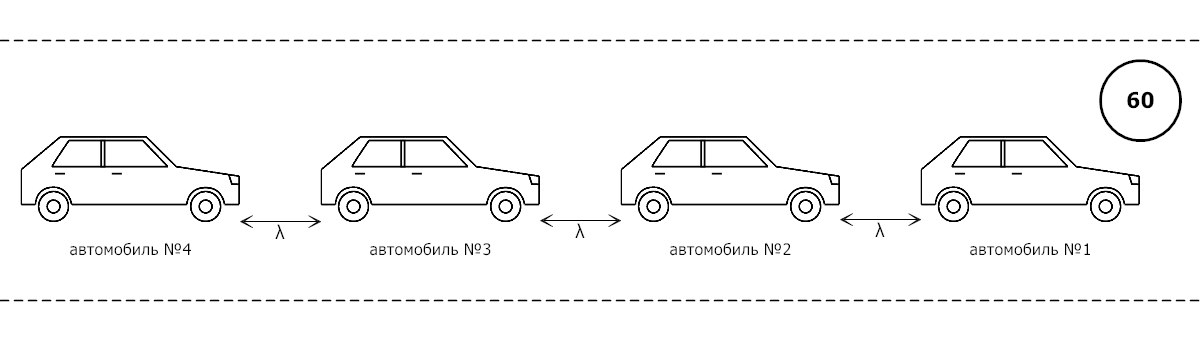
\includegraphics[keepaspectratio,width=160mm,height=70mm]{Images/car's_start_position.png}
	\end{center}
	\caption{Автомобили в момент старта.}
	\label{car's_start_position}
\end{figure}

Наибольшее влияние на проходимость транспортных средств через светофор оказываю мощность транспортного средства $d$ и время реакции водителя $\tau$, поэтому для различных значений этих параметров для системы \eqref{equation_without_stopping}. составлена таблица \eqref{table_without_stopping}. В этой таблице приведено количество транспортных средств, которые пройдут через светофор за время $t=40$ и будут соблюдать безопасную дистанцию $\lambda = 150$.  
 
\begin{table}[h!]
	\caption{Количество транспортных средств для модели \eqref{equation_without_stopping}}
	\label{table_without_stopping}
	\begin{center}
		\begin{tabular}{|l|*{5}{c|}}\hline
			\backslashbox{$d$}{$\tau$}
			&\makebox[3em]{1}&\makebox[3em]{2}&\makebox[3em]{3}	&\makebox[3em]{4}&\makebox[3em]{5}
			\\\hline
			0.1 &3&3&3&3&2
			\\\hline
			0.5 &7&6&5&5&4
			\\\hline
			1 &9&7&6&6&5
			\\\hline
			2 &10&8&7&6&5
			\\\hline
			3 &11&9&7&6&5
			\\\hline
		\end{tabular}
	\end{center}
\end{table} 

В таблице \eqref{table_with_stopping} приведено количество транспортных средств для системы \eqref{equation_with_stopping}, в которой время $t=40$ безопасная дистанция $\lambda = 150$, а время начала остановки $t_s=20$. 

\begin{table}[h!]
	\caption{Количество транспортных средств для модели \eqref{equation_with_stopping}}
	\label{table_with_stopping}
	\begin{center}
		\begin{tabular}{|l|*{5}{c|}}\hline
			\backslashbox{$d$}{$\tau$}
			&\makebox[3em]{1}&\makebox[3em]{2}&\makebox[3em]{3}	&\makebox[3em]{4}&\makebox[3em]{5}
			\\\hline
			0.1 &3&2&2&2&1
			\\\hline
			0.5 &7&5&5&3&2
			\\\hline
			1 &9&6&5&4&2
			\\\hline
			2 &10&7&6&5&3
			\\\hline
			3 &11&10&7&6&4
			\\\hline
		\end{tabular}
	\end{center}
\end{table} 
 
В таблицах \eqref{table_without_stopping} и \eqref{table_with_stopping} приведены данные для каких-то значений, немеющих ничего общего с реальными данными, но и из них отчётливо видно, что проходимость транспортного потока различна при различных параметрах и может быть оптимизирована. Изучение реальных параметров и подстановка их в модели \eqref{equation_without_stopping} и \eqref{equation_with_stopping} даст точный результат, позволит смоделировать реальную жизненную ситуацию и поможет оптимизировать технологии управления транспортными потоками.

\vspace{\baselineskip} \vspace{\baselineskip} \vspace{\baselineskip} 
\vspace{\baselineskip} \vspace{\baselineskip} \vspace{\baselineskip}
\hspace{0pt}

\newpage
\section*{Заключение}
\addcontentsline{toc}{section}{Заключение}
На основе проведённых исследований можно сделать вывод, что теоретический подход, основанный на принципе следования транспортных средств друг за другом, позволяет построить содержательную математическую модель для описания движения транспортных потоков. С использованием этого теоретического подхода было построено две математические модели  \eqref{equation_without_stopping} и \eqref{equation_with_stopping}, которые имеют большую прикладную значимость. На основе этих моделей можно исследовать различные жизненные ситуации, например, смоделировать начало движения автомобилей, найти оптимальную проходимость транспортных средств через светофор и множество других аналогичных ситуаций. Все исследования можно проводить с использованием компьютерных технологий, что позволит сделать технологии управления дорожным движением более современными.

\newpage

\begin{thebibliography}{**}
	\bibitem{Street}
	Дубелиръ Г.Д. "Городскiя улицы и мостовыя". 1912.
	
	\bibitem{TrafficFlow}
	https://spravochnick.ru/logistika/logisticheskie\_potoki/transportnyy\_potok/
	
	\bibitem{GippsModel}
	Wilson R. E. Gipps’ Model of Highway Traffic. 2002.
	
	\bibitem{FirstFollowTheLeaderModel}
	Pipes L.A. An operational analysis of traffic dynamics. 1953. 
	
	\bibitem{RefineFirstFollowTheLeaderModel}
	Chandler R.E., Herman R., Montroll E.W. Traffic dynamics: Studies in car following. 1958.
	
	\bibitem{Course}
	Погребняк М.А. Курсовая работа по теме "Математическое моделирование движения транспортных потоков". 2019.
	
	\bibitem{GazisModel}
	Gazis D.C., Herman R., Rothery R.W. Nonlinear follow the leader models of traffic
flow. 1961.

	
	\bibitem{StudyingGazisModel_1}
	May, Jr. A.D., Kel ler H.E.M. Non-integer car-following models. 1967.
	
	\bibitem{StudyingGazisModel_2}
	K\"{u}hne R.D., R\"{o}diger M.B. Ma
ros
opi
 simulation model for freeway traffic with jams
	and stop-start waves. 1991.
	
	\bibitem{StudyingGazisModel_3}
	K\"{u}hne R.D., Kroen A. Knowledge-based optimization of line 
ontrol systems for freeways. 1992.

%	\bibitem{Polygon}
%	Выгодский М.Я. Справочник по элементарной математике. 2001.
% 	\bibitem{Runge_Kutta}
%	 Бахвалов Н.С.  Численные методы. 1975.  
%	\bibitem{Refactoring}
%	Мартин Ф. Рефакторинг. Улучшение существующего кода. 2008.
	\bibitem{Gost}
	"ГОСТ Р 52289-2004. Национальный стандарт Российской Федерации. Технические средства организации дорожного движения. Правила применения дорожных знаков, разметки, светофоров, дорожных ограждений и направляющих устройств" (утв. Приказом Ростехрегулирования от 15.12.2004 N 120-ст) (ред. от 09.12.2013)
	\bibitem{News}
	https://www.yar.kp.ru/daily/26801.4/3835277/
\end{thebibliography}

\end{document}